\chapter{Конструкторская часть}

В данной части будет представлена схема проектируемой базы данных, будут описаны сущности базы данных, ограничения целостности, ролевая модель и используемые функции и триггеры.

\section{Диаграмма проектируемой базы данных}

На рисунке \ref{img:scheme} представлена диаграмма проектируемой базы данных.

\begin{figure}[H]
	\centering
	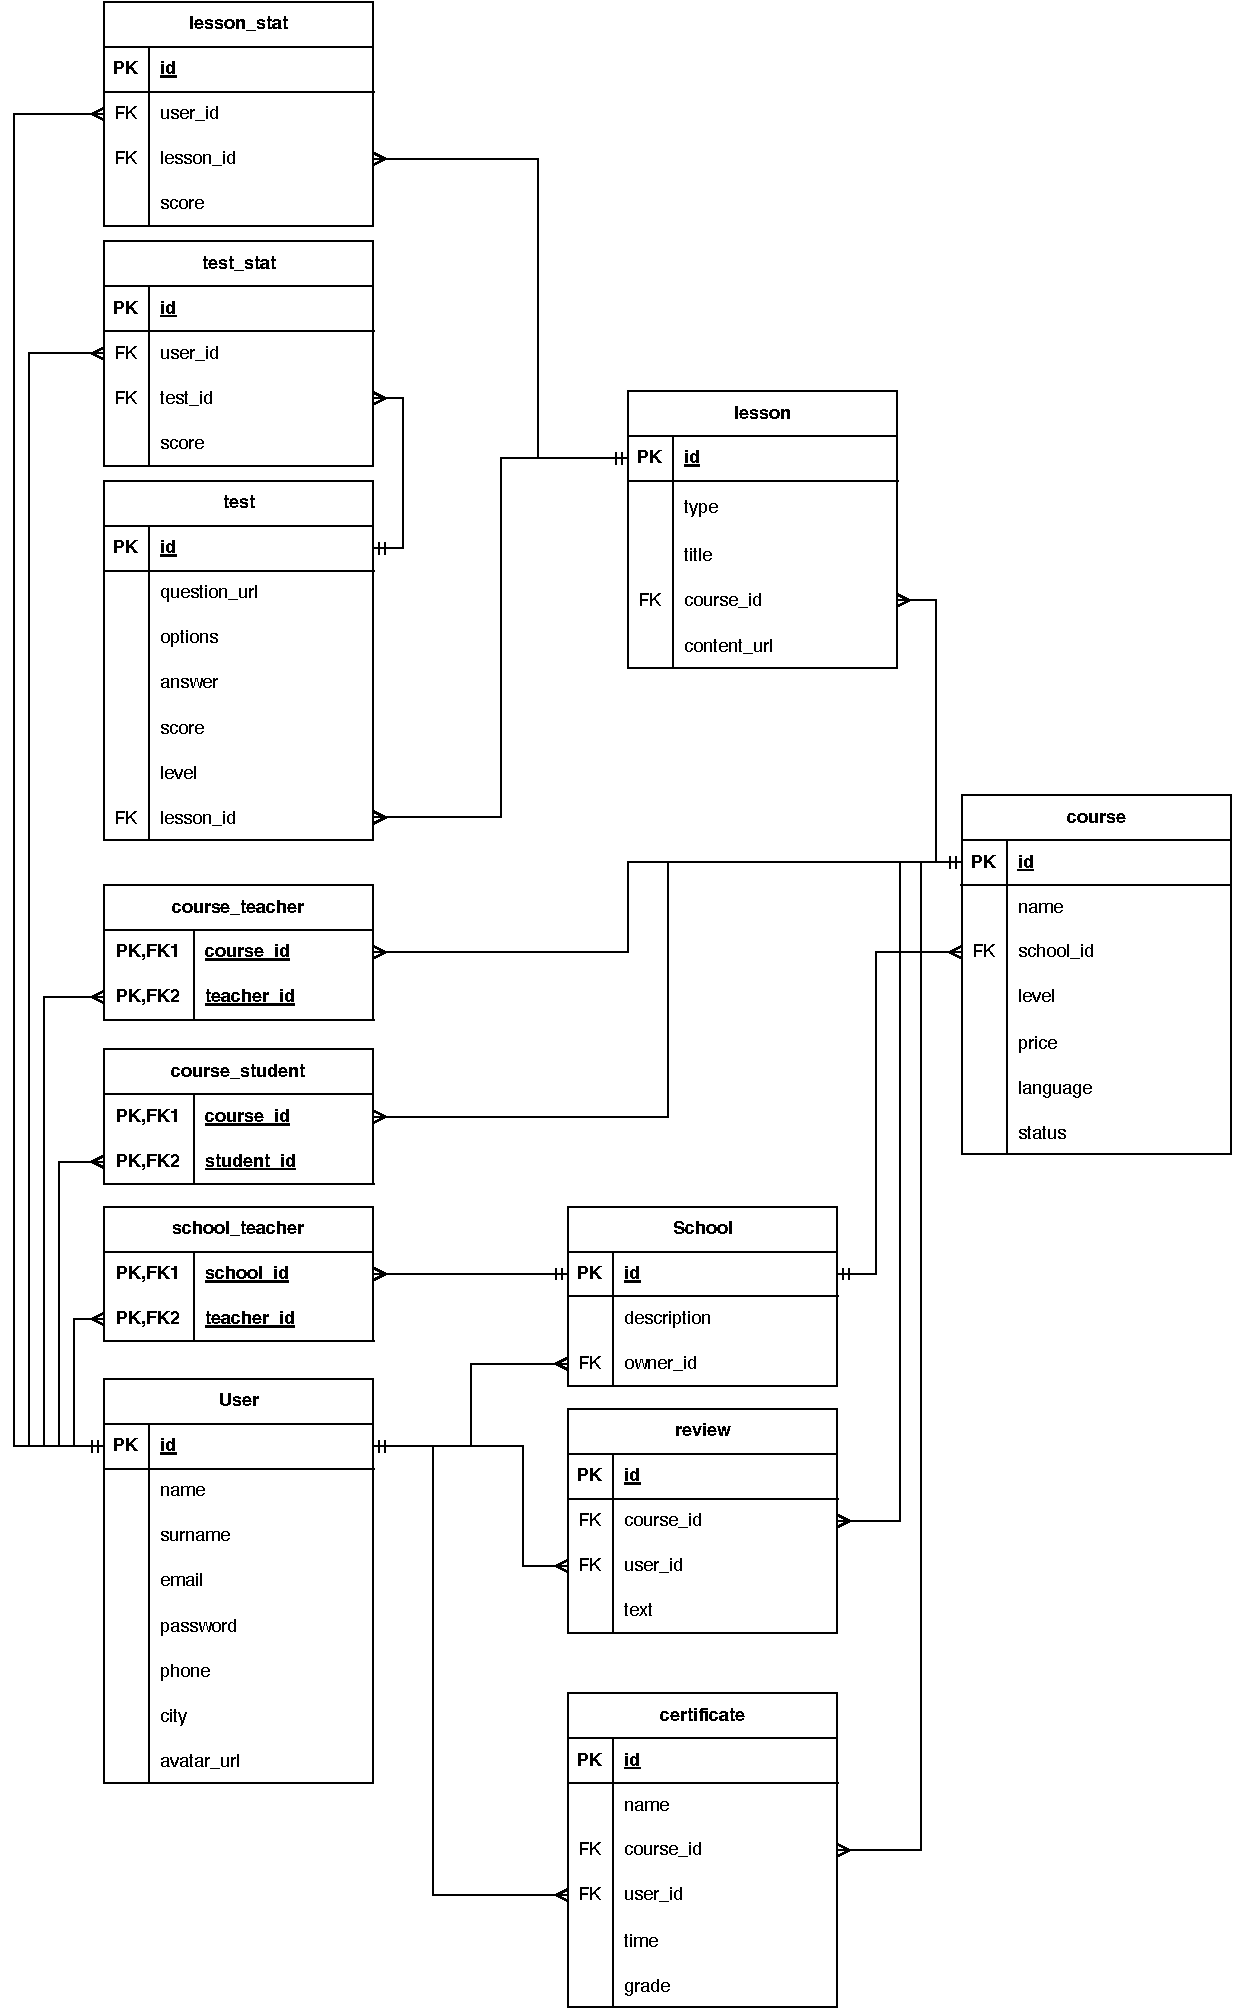
\includegraphics[height=0.9\textheight]{inc/img/scheme.pdf}
	\caption{Диаграмма проектируемой базы данных}
	\label{img:scheme}
\end{figure}

\section{Описание сущностей базы данных}


\begin{table}[H]
	\caption{\label{tbl:user}Поля таблицы user}
	\resizebox{\textwidth}{!}{
	\def\arraystretch{1}
	\begin{tabular}{|l|l|l|l|}
	\hline
	Поле        & Тип данных   & Ограничения целостности & Описание                      \\ \hline
	id          & uuid         & primary key             & Идентификатор пользователя    \\ \hline
	email       & varchar(255) & unique not null         & Почта пользователя            \\ \hline
	password    & varchar(255) & not null                & Пароль пользователя           \\ \hline
	name        & varchar(255) & not null                & Имя пользователя              \\ \hline
	surname     & varchar(255) & not null                & Фамилия пользователя          \\ \hline
	phone       & varchar(255) & нет                     & Номер телефона пользователя   \\ \hline
	city        & varchar(255) & нет                     & Город пользователя            \\ \hline
	avatar\_url & text         & нет                     & Ссылка на аватар пользователя \\ \hline
	\end{tabular}
	}
\end{table}

\begin{table}[H]
	\caption{\label{tbl:school}Поля таблицы school}
	\resizebox{\textwidth}{!}{
	\def\arraystretch{1}
	\begin{tabular}{|l|l|l|l|}
	\hline
	Поле        & Тип данных   & Ограничения целостности & Описание                      \\ \hline
	id          & uuid         & primary key             & Идентификатор школы    \\ \hline
	name        & varchar(255) & not null                & Название школы                \\ \hline
	description & text         & not null                & Описание школы                \\ \hline
	owner\_id   & uuid         & not null                & Идентификатор владельца школы \\ \hline
	\end{tabular}
	}
\end{table}

\begin{table}[H]
	\caption{\label{tbl:course}Поля таблицы course}
	\resizebox{\textwidth}{!}{
	\def\arraystretch{1}
	\begin{tabular}{|l|l|l|l|}
	\hline
	Поле       & Тип данных     & Ограничения целостности & Описание                                                                        \\ \hline
	id         & uuid           & primary key             & Идентификатор курса                                                             \\ \hline
	name       & varchar(255)   & not null                & Название курса                                                                  \\ \hline
	school\_id & uuid           & not null                & \begin{tabular}[c]{@{}l@{}}Идентификатор школы,\\ владеющей курсом\end{tabular} \\ \hline
	level      & int            & not null                & Уровень сложности курса                                                         \\ \hline
	price      & bigint         & not null                & Цена курса                                                                      \\ \hline
	language   & varchar(255)   & not null                & Язык материала курса                                                            \\ \hline
	status     & course\_status & not null                & Текущий статус курса                                                            \\ \hline
	rating     & float          & not null                & Пользовательская средняя оценка курса                                                   \\ \hline
	\end{tabular}
	}
\end{table}

Поле status таблицы school имеет перечисляемый тип данных и может принимать три варианта: <<draft>>, <<ready>>, <<published>>. Статус курса -- текущее состояние готовности и наполнения материалом курса. Черновик курса может редактироваться автором, после чего может быть переведен в состояние готовности к публикации. После успешной публикации курса, состояние меняется на <<опубликован>>.

\begin{table}[H]
	\caption{\label{tbl:lesson}Поля таблицы lesson}
	\resizebox{\textwidth}{!}{
	\def\arraystretch{1}
	\begin{tabular}{|l|l|l|l|}
	\hline
	Поле        & Тип данных   & Ограничения целостности & Описание                                                                             \\ \hline
	id          & uuid         & primary key             & Идентификатор урока                                                                  \\ \hline
	title       & varchar(255) & not null                & Название урока                                                                       \\ \hline
	type        & lesson\_type & not null                & Тип урока                                                                            \\ \hline
	score       & int          & not null                & Максимальная оценка за урок                                                          \\ \hline
	theory\_url & text         & нет                     & \begin{tabular}[c]{@{}l@{}}Ссылка на теоретический \\ материал урока\end{tabular}    \\ \hline
	video\_url  & text         & нет                     & Ссылка на видео материал урока                                                       \\ \hline
	course\_id  & uuid         & not null                & \begin{tabular}[c]{@{}l@{}}Идентификатор курса,\\ который содержит урок\end{tabular} \\ \hline
	\end{tabular}
	}
\end{table}

Урок может быть трех видов: теоретический, видео-урок и практический урок. Тип урока описывается полем type таблицы lesson и может принимать значения: <<theory>>, <<video>>, <<practice>>.

\begin{table}[H]
	\caption{\label{tbl:test}Поля таблицы test}
	\resizebox{\textwidth}{!}{
	\def\arraystretch{1}
	\begin{tabular}{|l|l|l|l|}
	\hline
	Поле       & Тип данных & Ограничения целостности & Описание                                                                            \\ \hline
	id         & uuid       & primary key             & Идентификатор теста                                                                 \\ \hline
	task\_url  & text       & not null                & \begin{tabular}[c]{@{}l@{}}Ссылка на описание \\ задачи теста\end{tabular}          \\ \hline
	options    & text       & not null                & Возможные варианты ответа                                                           \\ \hline
	answer     & text       & not null                & Ответ на задание                                                                    \\ \hline
	score      & int        & not null                & \begin{tabular}[c]{@{}l@{}}Максимальная оценка за \\ прохождение теста\end{tabular} \\ \hline
	level      & int        & not null                & Уровень сложности теста                                                             \\ \hline
	lesson\_id & uuid       & not null                & \begin{tabular}[c]{@{}l@{}}Идентификатор урока, \\ содержащего тест\end{tabular}    \\ \hline
	\end{tabular}
	}
\end{table}

\begin{table}[H]
	\caption{\label{tbl:review}Поля таблицы review}
	\resizebox{\textwidth}{!}{
	\def\arraystretch{1}
	\begin{tabular}{|l|l|l|l|}
	\hline
	Поле       & Тип данных & Ограничения целостности & Описание                      \\ \hline
	id         & uuid       & primary key             & Идентификатор отзыва об уроке \\ \hline
	text       & text       & not null                & Текст отзыва об уроке         \\ \hline
	course\_id & uuid       & not null                & Идентификатор курса           \\ \hline
	user\_id   & uuid       & нет                     & Идентификатор пользователя    \\ \hline
	rating     & int        & нет                     & Оценка курса                  \\ \hline
	\end{tabular}
	}
\end{table}

\begin{table}[H]
	\caption{\label{tbl:certificate}Поля таблицы certificate}
	\resizebox{\textwidth}{!}{
	\def\arraystretch{1}
	\begin{tabular}{|l|l|l|l|}
	\hline
	Поле        & Тип данных         & Ограничения целостности & Описание                          \\ \hline
	id          & uuid               & primary key             & Идентификатор отзыва об уроке     \\ \hline
	name        & varchar(1024)      & not null                & Название сертификата              \\ \hline
	score       & int                & not null                & Итоговая оценка прохождения курса \\ \hline
	grade       & certificate\_grade & not null                & Степень сертификата               \\ \hline
	created\_at & timestamp          & not null                & Дата выдачи сертификата           \\ \hline
	user\_id    & uuid               & not null                & Идентификатор пользователя        \\ \hline
	course\_id  & uuid               & нет                     & Идентификатор курса               \\ \hline
	\end{tabular}
	}
\end{table}

Сертификаты могут быть трех видов: бронзовый, серебряный и золотой. Тип сертификата описывается полем grade таблицы certificate и может принимать значения: <<bronze>>, <<silver>>, <<gold>>.

\begin{table}[H]
	\caption{\label{tbl:lesson_stat}Поля таблицы lesson\_stat}
	\resizebox{\textwidth}{!}{
	\def\arraystretch{1}
	\begin{tabular}{|l|l|l|l|}
	\hline
	Поле       & Тип данных & Ограничения целостности & Описание                                                                                       \\ \hline
	id         & uuid       & primary key             & \begin{tabular}[c]{@{}l@{}}Идентификатор записи о \\ результате прохождения урока\end{tabular} \\ \hline
	score      & int        & not null                & Оценка прохождения урока                                                                       \\ \hline
	user\_id   & uuid       & not null                & Идентификатор пользователя                                                                     \\ \hline
	lesson\_id & uuid       & not null                & Идентификатор урока                                                                            \\ \hline
	\end{tabular}
	}
\end{table}

\begin{table}[H]
	\caption{\label{tbl:test_stat}Поля таблицы test\_stat}
	\resizebox{\textwidth}{!}{
	\def\arraystretch{1}
	\begin{tabular}{|l|l|l|l|}
	\hline
	Поле     & Тип данных & Ограничения целостности & Описание                                                                                       \\ \hline
	id       & uuid       & primary key             & \begin{tabular}[c]{@{}l@{}}Идентификатор записи о \\ результате прохождения урока\end{tabular} \\ \hline
	score    & int        & not null                & Оценка прохождения урока                                                                       \\ \hline
	user\_id & uuid       & not null                & Идентификатор пользователя                                                                     \\ \hline
	test\_id & uuid       & not null                & Идентификатор тест                                                                             \\ \hline
	\end{tabular}
	}
\end{table}

Таблицы lesson\_stat и test\_stat хранят данные о прохождении пользователем уроков и тестов соответственно. Сертификат о прохождении курса формируется на основании информации из этих таблиц. 

\begin{table}[H]
	\caption{\label{tbl:course_student}Поля таблицы course\_student}
	\resizebox{\textwidth}{!}{
	\def\arraystretch{1}
	\begin{tabular}{|l|l|l|l|}
	\hline
	Поле        & Тип данных & Ограничения целостности & Описание                   \\ \hline
	student\_id & uuid       & not null                & Идентификатор пользователя \\ \hline
	course\_id  & uuid       & not null                & Идентификатор курса        \\ \hline
	\end{tabular}
	}
\end{table}

\begin{table}[H]
	\caption{\label{tbl:course_teacher}Поля таблицы course\_teacher}
	\resizebox{\textwidth}{!}{
	\def\arraystretch{1}
	\begin{tabular}{|l|l|l|l|}
	\hline
	Поле        & Тип данных & Ограничения целостности & Описание                   \\ \hline
	teacher\_id & uuid       & not null                & Идентификатор пользователя \\ \hline
	course\_id  & uuid       & not null                & Идентификатор курса        \\ \hline
	\end{tabular}
	}
\end{table}

\begin{table}[H]
	\caption{\label{tbl:school_teacher}Поля таблицы school\_teacher}
	\resizebox{\textwidth}{!}{
	\def\arraystretch{1}
	\begin{tabular}{|l|l|l|l|}
	\hline
	Поле        & Тип данных & Ограничения целостности & Описание                   \\ \hline
	teacher\_id & uuid       & not null                & Идентификатор пользователя \\ \hline
	school\_id  & uuid       & not null                & Идентификатор школы        \\ \hline
	\end{tabular}
	}
\end{table}

Таблица course\_student является развязочной для курсов и обучающихся на них студентах. Развязочная таблица course\_teacher связывает курсы и их преподавателей, а таблица school\_teacher является развязочной для школ и их преподавателей.

\section{Ролевая модель}

В данной работе выделяются следующие роли:
\begin{itemize}
	\item гость -- имеет возможность просматривать курсы, школы и их преподавателей, отзывы о курсах;
	\item пользователь -- имеет права на просмотр, редактирование и удаление собственных курсов, школ, уроков, тестов, а также может проходить приобретенные курсы;
	\item администратор -- имеет все права для действий со всеми таблицами.
\end{itemize}

\section{Триггер базы данных}

К каждому курсу пользователи, прошедшие данный курс, могут оставить отзыв и выставить оценку качества. При этом средняя оценка курса должна меняться при операциях над таблицей отзывов. Для этого используется триггер базы данных, который сработает при добавлении, удалении или обновлении отзыва пользователя. Таким образов, средняя оценка пересчитывается и при получении информации о курсе исчезает необходимость пересчитывать ее каждый раз.

На рисунке \ref{img:trigger} представлена схема алгоритма триггера для пересчета средней оценки курса.

\begin{figure}[H]
	\centering
	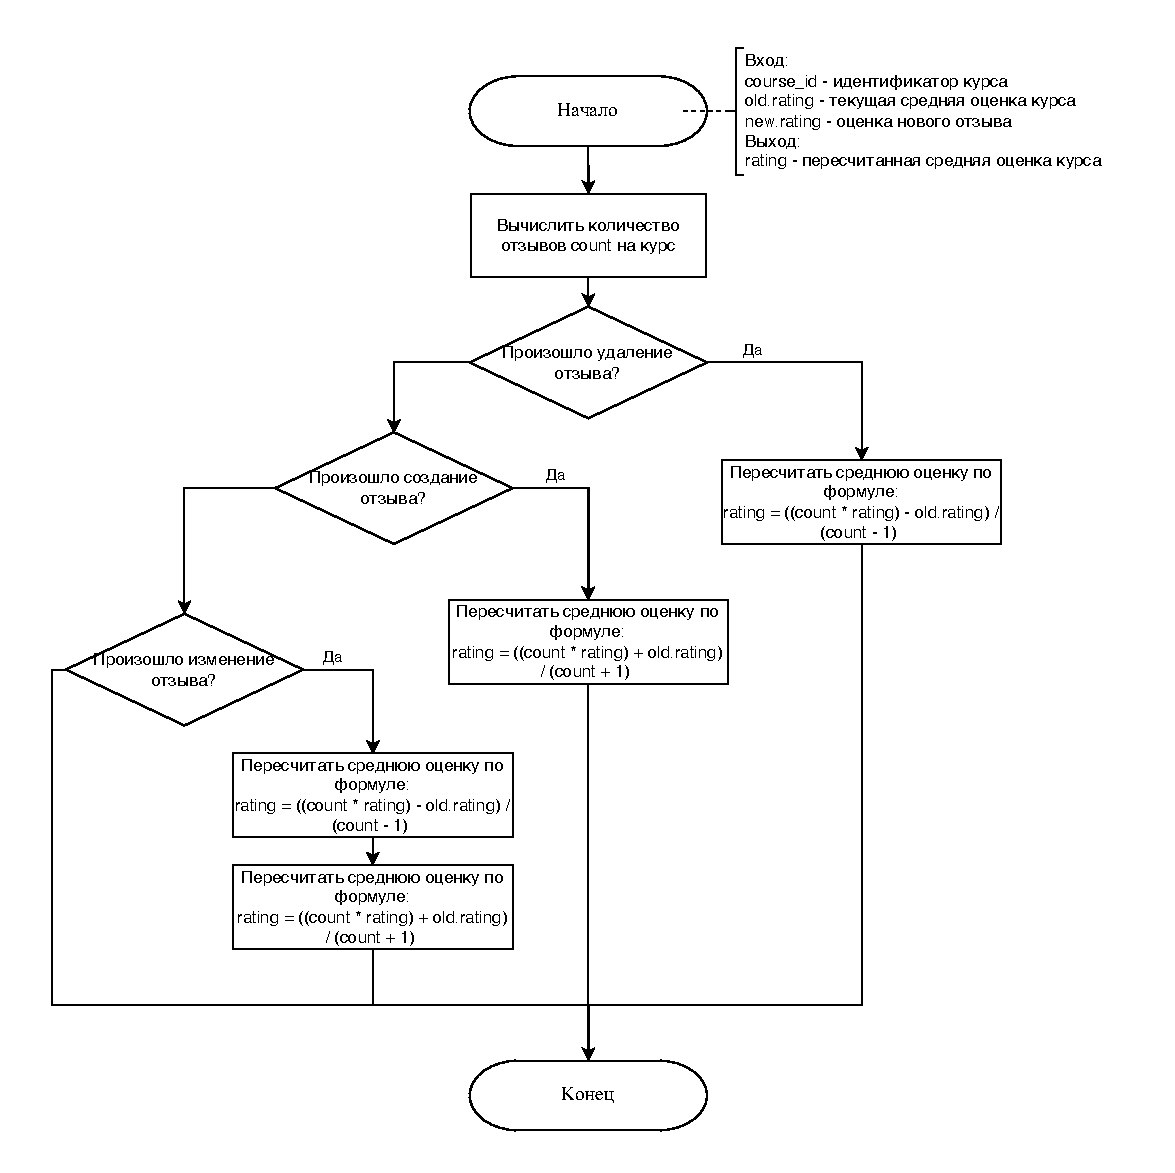
\includegraphics[height=0.7\textheight]{inc/img/trigger.pdf}
	\caption{Схема алгоритма триггера}
	\label{img:trigger}
\end{figure}

\section{Вывод из конструкторской части}

В данной части были спроектирована схема базы данных, описаны сущности базы данных, ограничения целостности, ролевая модель и используемые функции и триггеры.
